\documentclass[12pt,a4paper]{article}
\usepackage[utf8x]{inputenc}
\usepackage{ucs}
\usepackage{amsmath}
\usepackage{amsfonts}
\usepackage{amssymb}
\usepackage{graphicx}
\usepackage{grffile}
\usepackage{float}
\usepackage[portuguese]{babel}
\title{Trabalho 6}
\author{André Garnier Coutinho}
\setlength{\textwidth}{17cm}
\setlength{\textheight}{24cm}
\addtolength{\topmargin}{-2cm}
\addtolength{\oddsidemargin}{-2cm}
\begin{document}
\begin{center}
\textbf{Instituto de Matemática e Estatística da USP\linebreak MAT 2455 - Cálculo Diferencial e Integral III para Engenharia\linebreak Trabalho 6 - 1º semestre de 2015}
\end{center}



\noindent{\bf Questão 1.} (2,5 pontos) Seja $S$ a parte da esfera $x^2 + y^2 + z^2 = 2z$, com $x \geq 0$. Calcule o fluxo do campo $\vec{F}(x,y,z) = (zx+2, cos(x^2), xz^2)$ através de $S$ orientada com a normal exterior a esfera.

\noindent{\bf \\Solução:}

Seja $S_1$ a superfície plana que fecha a superfície $S$. Como o domínio de $\vec{F} $ não apresenta singularidades na região $V$ definida pelo interior de $S \cup S_1 $, e orientando para fora a normal da superfície fechada $S \cup S_1$ , pelo Teorema de Gauss:

$$ \iint_{S} \vec{F}  \cdot \vec{N} \,dS + \int_{ S_1 } \vec{F}  \cdot \vec{N} \,dS = \iiint_{V} div(\vec{F})  \,dx \,dy \,dz $$

\begin{equation}
\iint_{S} \vec{F}  \cdot \vec{N} \,dS = - \iint_{ S_1 } \vec{F}   \cdot \vec{N} \,dS  + \iiint_{V} div(\vec{F}) \,dx \,dy \,dz
\label{eq:1}
\end{equation} \\


\begin{figure}[h!]
	\centering
	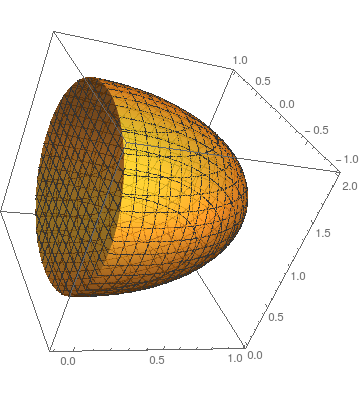
\includegraphics[scale=0.5]{figura1.png}  
	\caption{Região V e superfícies $S$ e $S_1$ }
	\label{fig:figura1}
\end{figure}

A superfície $S_1$ pode ser facilmente parametrizada da seguinte forma:

\[ \sigma (u,v) = (0, u, v) \] 

Para encontrar os valores de $(u,v)$ em que a superfície $S_1$ é definida, encontramos a intersecção do plano $x=0$ com a esfera. Assim temos:

$$ \begin{cases}
x = 0 \\
x^2 + y^2 + z^2 = 2z
\end{cases}
\Rightarrow y^2 + (z-1)^2 = 1
$$

Sendo assim, temos que a região $R$ na qual a superfície $S_1$ é definida é:
$$ R = \{ (u,v) \in \mathbb{R}^2 \hspace{1 mm} | \hspace{1 mm}  u^2 + (v-1)^2 \leq 1 \} $$

Calculando o vetor $\sigma_u \wedge \sigma_v$:

\[ \sigma_u = (0,1, 0 ) \]
\[ \sigma_v = (0,0, 1 ) \]
\[  \sigma_u \wedge \sigma_v = ( 1, 0, 0 ) \] 

Como a normal da superfície $S_1$ é para baixo e $\sigma_u \wedge \sigma_v$ é oposta ao eixo $x$, invertemos o sinal de $\sigma_u \wedge \sigma_v$ para calcular a integral de superfície. Assim:
$$ \iint_{S_1} \vec{F}  \cdot \vec{N} \,dS = \iint_{R} (0 + 2 , \cos(0), 0 ) \cdot (-1, 0, 0) \,du \,dv = -2 \iint_{R}   \,du \,dv  $$

Como a região $R$ é um disco de raio $1$:


\begin{equation}
\iint_{S_1} \vec{F}  \cdot \vec{N} \,dS = -2\pi
\label{eq:2}
\end{equation}

$$ div(\vec{F}) =  \frac{\partial P}{\partial x} + \frac{\partial Q}{\partial y} + \frac{\partial R}{\partial z}  = z + 0 + 2x =  z(1+2x) $$

Realizando a seguinte mudança para coordenadas esféricas:
\begin{equation}
\begin{cases}
x = \rho\sin\phi\cos\theta\\
y = \rho\sin\phi\sin\theta\\ 
z = \rho\cos\phi + 1\\
\end{cases}
\label{eq:mudanca}
\end{equation}
$$ |J| = \rho^2 \sin\phi $$
$$ \iiint_{V} div(\vec{F}) \,dx \,dy \,dz = \int_{-\frac{\pi}{2}}^{\frac{\pi}{2}} \int_{0}^{\pi} \int_{0}^{1} (1 + \rho\cos\phi)(1 + 2\rho\sin\phi\cos\theta)\rho^2 \sin\phi \,d\rho \,d\phi \,d\theta $$
$$ =  \int_{-\frac{\pi}{2}}^{\frac{\pi}{2}} \int_{0}^{\pi} \int_{0}^{1} ( \rho^2 \sin\phi + 2 \rho^3\sin^2\phi\cos\theta + \rho^3\sin\phi\cos\theta + 2\rho^4\sin^2\phi\cos\phi\cos\theta )  \,d\rho \,d\phi \,d\theta  $$
$$ =  \int_{-\frac{\pi}{2}}^{\frac{\pi}{2}} \int_{0}^{\pi} \Big(  \frac{\sin\phi}{3} +  \frac{\sin^2\phi\cos\theta}{2} + \frac{\sin\phi\cos\theta}{4} + \frac{2\sin^2\phi\cos\phi\cos\theta}{5} \Big) \,d\phi \,d\theta  $$
$$ =  \int_{-\frac{\pi}{2}}^{\frac{\pi}{2}} \int_{0}^{\pi} \Big(  \frac{\sin\phi}{3} +  \Big( \frac{1 - \cos(2\phi)}{2} \Big) \frac{\cos\theta}{2} + \frac{\sin(2\phi)}{8} + \frac{2\sin^2\phi\cos\phi\cos\theta}{5} \Big) \,d\phi \,d\theta  $$
$$ =  \int_{-\frac{\pi}{2}}^{\frac{\pi}{2}} \Big( - \frac{\cos\phi}{3} +  \Big( \phi - \frac{ \sin(2\phi)}{2} \Big) \frac{\cos\theta}{4} - \frac{\cos(2\phi)}{16} + \frac{2}{5} \frac{\sin^3\phi\cos\theta}{3} \Big)_{\phi=0}^{\phi=\pi}  \,d\theta $$
$$ =  \int_{-\frac{\pi}{2}}^{\frac{\pi}{2}} \Big(  \frac{2}{3} +  \frac{\pi\cos\theta}{4}  \Big) \,d\theta =  \Big(  \frac{2\theta}{3} +  \frac{\pi\sin\theta}{4}  \Big)_{-\frac{\pi}{2}}^{\frac{\pi}{2}} = \frac{7\pi}{6} $$
\begin{equation}
\therefore \iiint_{V} div(\vec{F}) \,dx \,dy \,dz = \frac{7\pi}{6}
\label{eq:3}
\end{equation} \\

Substituindo (\ref{eq:2}) e (\ref{eq:3}) em (\ref{eq:1}):

$$ \iint_{S} \vec{F} \cdot \vec{N} \,dS = -2\pi + \frac{7\pi}{6} = -\frac{5\pi}{6}  $$
 
\newpage

\noindent{\bf Questão 2.} (3 pontos) Calcule $\displaystyle\int_{\gamma} \frac{-y}{x^2 + y^2}dx + \frac{x}{x^2 + y^2}dy + (x + e^{z^2})dz$, sendo $\gamma$ a curva dada pela intersecção de $z = 5 - y^2$ e $z = x^2 + 2x + y^2 -3$, orientada de modo que sua projeção no plano $xy$ é percorrida no sentido anti-horário.

Sugestão: Escreva o campo $\vec{F}$ como $\vec{F_1} + (0,0,x)$.

\noindent{\bf \\Solução:}

Podemos decompor $\vec{F}$ na soma de dois campos vetoriais $\vec{F_1}$ e $\vec{F_2}$, sendo:

$$ \vec{F_1} =  \Big( \frac{-y}{x^2 + y^2}, \frac{x}{x^2 + y^2}, e^{z^2} \Big) ; \vec{F_2} = ( 0, 0, x ) $$

Calculando os rotacionais de $\vec{F_1}$ e $\vec{F_2}$:

$$ \displaystyle Rot(\vec{F_1}) =
\begin{vmatrix}
\vec{i} & \vec{j} & \vec{k} \\
\frac{\partial}{\partial x} & \frac{\partial}{\partial y} & \frac{\partial}{\partial z}  \\
\frac{-y}{x^2 + y^2}  & \frac{x}{x^2 + y^2} & e^{z^2}
\end{vmatrix} 
= \Big( \frac{1 \cdot (x^2 + y^2) - x \cdot (2x)}{(x^2 + y^2)^2} - \frac{(-1) \cdot (x^2 + y^2) - (-y) \cdot (2y)}{(x^2 + y^2)^2} \Big) \vec{k} = \vec{0} $$

$$ Rot(\vec{F_2}) =
\begin{vmatrix} \vec{i} & \vec{j} & \vec{k} \\
\frac{\partial}{\partial x} & \frac{\partial}{\partial y} & \frac{\partial}{\partial z}  \\
0 & 0 & x
\end{vmatrix} = -\vec{j} $$

Como $\gamma$ é uma curva fechada e o domínio de $\vec{F_2}$ é simplesmente conexo, podemos utilizar o teorema de Stokes para calcular $ \displaystyle \int_{\gamma} \vec{F_2} \cdot d\vec{r} $, escolhendo como superfície  $z = 5 - y^2$ limitada por $z = x^2 + 2x + y^2 -3$, a qual chamaremos de $S_2$ . \\

Como a projeção de $\gamma $ em $0xy$ é no sentido anti-horário, temos que a normal induzida pelo Teorema de Stokes em $S_2$ tem a componente na direção $\vec{k}$ positiva. Assim, parametrizando $S_2$:
$$ \sigma (u,v) = (u,v, 5-v^2) $$
Para encontrar os valores de $(u,v)$ em que a superfície $S_2$ é definida, encontramos a intersecção da calha com o parabolóide. Assim temos:

$$\begin{cases}
z = 5 - y^2 \\
z = x^2 + 2x + y^2 - 3
\end{cases}
\Rightarrow
5 - y^2 = x^2 + 2x + y^2 - 3 \Rightarrow (x+1)^2 + 2y^2 = 9 $$

Sendo assim, temos que a região $R_2$ na qual a superfície $S_2$ é definida é: \\
$$ R_2 = \{ (u,v) \in \mathbb{R}^2 \hspace{1 mm} | \hspace{1 mm}  (u+1)^2 + 2v^2 \leq 9 \} $$

Calculando o vetor $\sigma_{u} \wedge \sigma_{v}$:
$$ \sigma_u = (1,0, 0 ) $$
$$ \sigma_v = (0,1, -2v ) $$
$$  \sigma_u \wedge \sigma_v = (0 , 2v, 1 ) $$
Como $\sigma_u \wedge \sigma_v$ está no mesmo sentido da normal de $S_2$, aplicando o Teorema de Stokes, temos:

$$ \int_{\gamma} \vec{F_2} \cdot d\vec{r} = \iint_{S_2} Rot(\vec{F_2}) \cdot \vec{N} \,dS = \iint_{R_2} ( 0, -1, 0 )  \cdot ( 0, 2v, 1 )  \,du \,dv = -2 \iint_{R_2} v \,du \,dv $$

Como a região $R_2$ é simetríca em $v$ e o integrando é uma função ímpar em $v$:

$$ \iint_{R_2} v \,du \,dv\ = 0 \Rightarrow  \int_{\gamma} \vec{F_2} \cdot d\vec{r} = 0 $$

Assim, como $ \displaystyle  \int_{\gamma} \vec{F} \cdot d\vec{r} =  \int_{\gamma} \vec{F_1} \cdot d\vec{r} +  \int_{\gamma} \vec{F_2} \cdot d\vec{r} $, temos que $ \displaystyle \int_{\gamma} \vec{F} \cdot d\vec{r} =  \int_{\gamma} \vec{F_1} \cdot d\vec{r} $. \\

Para calcular $ \displaystyle \int_{\gamma} \vec{F_1} \cdot d\vec{r} $, não podemos escolher uma superfície que seja cortada pelo eixo $z$ quando aplicarmos o Teorema de Stokes, pois $\vec{F_1}$ não é definido para pontos do tipo $(0,0,z), z \in \mathbb{R} $.

Sendo assim, escolhemos a superfície cilindrica $(x+1)^2 + 2y^2 = 9$ limitada por $z = 0 $ e $z = 5 - y^2 $, a qual chamaremos de $S_1$ sendo $\gamma$ e $\gamma_1$ os bordos do cilindro. Como a projeção de $\gamma $ em $0xy$ é no sentido anti-horário, temos que a normal induzida pelo Teorema de Stokes em $S_1$ aponta para dentro do cilindro, o que induz uma orientação no sentido horário para $ \gamma_1$. Assim, aplicando o Teorema de Stokes:

$$ \int_{\gamma} \vec{F_1} \cdot d\vec{r} + \int_{\gamma_1} \vec{F_1} \cdot d\vec{r} = \iint_{S_1} Rot(\vec{F_1}) \cdot \vec{N} \,dS = 0 $$
$$ \therefore \int_{\gamma} \vec{F_1} \cdot d\vec{r} = - \int_{\gamma_1} \vec{F_1} \cdot d\vec{r} $$

A região do plano $xy$ interna a $\gamma_1$ contém o ponto $(0,0,0)$, o qual é uma singularidade de $\vec{F_1}$. Então adicionamos a curva $\gamma_2 (t) = ( \cos t, \sin t, 0), t \in [0, 2 \pi] $ a qual isola a singularidade e não se cruza com  $\gamma_1$.


Como $\gamma_1$ e $\gamma_2$ estão no sentido contrário ao induzido pelo Teorema de Green, para aplicar o teorema invertemos os sinais das integrais de linha. Assim, aplicando o teorema de Green:

$$ - \int_{\gamma_1} \vec{F_1} \cdot d\vec{r} - \int_{\gamma_2} \vec{F_1} \cdot d\vec{r} = \iint_{R} Rot(\vec{F_1}) \cdot \vec{k} \,dx \,dy = 0 $$
$$ \therefore \int_{\gamma_1} \vec{F_1} \cdot d\vec{r} = - \int_{\gamma_2} \vec{F_1} \cdot d\vec{r} = - \int_{0}^{2 \pi} \Big( \frac{-\sin t}{\cos^2 t + \sin^2 t} , \frac{\cos t }{\cos^2 t + \sin^2 t} , 1 \Big) \cdot (-\sin t , \cos t, 0 ) \,dt $$
$$ = - \int_{0}^{2 \pi} \Big( \sin^2 t +  \cos^2 t \Big) \,dt = - 2\pi $$
$$ \therefore \int_{\gamma} \vec{F} \cdot d\vec{r} = 2\pi $$

\newpage

\noindent{\bf Questão 3.} (1,5 ponto) Decida se cada afirmação a seguir é verdadeira ou falsa e justifique a resposta.

Nos itens $\vec{F}$ denota um campo qualquer definido num aberto conexo do $\mathbb{R}^3$ de classe $C^1$.

\begin{itemize}
	\item[1.] Se $div(\vec{F}) = 0$, então $\displaystyle\iint_{S} \vec{F} \cdot \vec{N} \,dS = 0$, para toda $S$ superfície fechada orientável.
	
	\item[2.] Se $\vec{F}$ é conservativo então $Rot(\vec{F}) = \vec{0}$.
	
	\item[3.] Se $Rot(\vec{F}) = \vec{0}$ então $div(\vec{F}) = 0$.

\end{itemize}


\noindent{\bf \\Solução:}

\begin{itemize}
	\item[1.] Afirmação falsa. Se $\vec{F}$ tiver singularidades no interior de $S$, não é possível aplicar o Teorema de Gauss diretamente, o que torna possível a integral não ser nula. Um exemplo disso é a integral do campo $\displaystyle\frac{x\vec{i} + y\vec{j} + z\vec{k}}{(\sqrt{x^2 + y^2 + z^2})^3}$ em uma esfera centrada em $(0,0,0)$.

	\item[2.] Afirmação verdadeira. Se $\vec{F}$ é convervativo, $\vec{F} = \nabla \phi $, logo:
	
	$$ Rot(\vec{F}) = Rot(\nabla\phi) = \begin{vmatrix}
	\vec{i} & \vec{j} & \vec{k} \\
	\frac{\partial}{\partial x} & \frac{\partial}{\partial y} & \frac{\partial}{\partial z} \\
	\frac{\partial \phi}{\partial x} & \frac{\partial \phi}{\partial y} & \frac{\partial \phi}{\partial z}
    \end{vmatrix} = \Big(\frac{\partial^2 \phi}{\partial y \partial z} - \frac{\partial^2 \phi}{\partial z \partial y} ,               \frac{\partial^2 \phi}{\partial z \partial x} - \frac{\partial^2 \phi}{\partial x \partial z}, \frac{\partial^2 \phi}{\partial x \partial y} - \frac{\partial^2 \phi}{\partial y \partial x}\Big)	 $$
    
    Como $\vec{F}$ é de classe $C^1$, como $\vec{F} = \nabla \phi $, $\phi$ é de classe $C^2$. Pelo Teorema de Clairaut-Schwarz, $\frac{\partial^2 f}{\partial x \partial y} = \frac{\partial^2 f}{\partial y \partial x}$, sendo $f(x,y)$ de classe $C^2$. Sendo assim, $Rot(\vec{F}) = \vec{0}$.
	
	\item[3.] Afirmação falsa. Seja $\vec{F} = x\vec{i}$, $Rot(\vec{F}) = \vec{0}$ e $div(\vec{F}) = 1$.

 \end{itemize}


\end{document}
